\section{Closed-form search: exploratory formulae}
\label{a:app:catalogue}

This appendix records the candidate formulae produced by the searches of
\cref{a:sec:GA}. They are approximations only, quarantined here because they are
not needed for the probabilistic role of $A(p)$ in the main text; they are
retained because they show how little a visually accurate fit says about the
singular quantity $1/A(p)$. These expressions have no inferential status: they are
records of a curve-fitting exercise, not proposed identities.

\subsection{Rational candidates}
\label{a:app:rational}

Polynomial and rational searches can be constrained to the known endpoints
$A(0)=\tfrac12$ and $A(\tfrac12)=0$. One of the more economical rational
candidates was
\begin{equation}
\widehat A_1(p)
=
\frac{\tfrac12(1-2p)(1+2p)}
     {1+\tfrac12p-\tfrac52p^2-\tfrac65p^3+\tfrac65p^4} ,
\label{a:eq:Ahat1}
\end{equation}
the candidate $\hat A_1$ of \cref{a:sec:GA}. It passes through both endpoints. At
the critical endpoint, however,
\begin{equation*}
\widehat A_1'\lrb{\tfrac12} = -\frac{2}{0.55}\approx-3.636,
\end{equation*}
whereas \cref{a:thm:nearcrit} requires the left derivative $-4$. Matching the
values but missing this slope is enough to make the relative error in $A$, and
hence the error in $1/A$, unacceptable near criticality.

\subsection{Tree-search candidates}
\label{a:app:treesearch}

A less restricted symbolic tree search over progressively nested elementary
functions produced many longer formulae of similar visual quality. Two
representative outputs were
\begin{multline}
\widehat A_2(p)
=0.31696448624690005
\ln\!\Biggl(
\Biggl|\cos\!\biggl(
\left(\frac{1}{3.19801133824532}\right)^{1/4}\\
{}+p\biggl[
\sin\!\Bigl(
  \cos\!\bigl(|p|(0.621865696665606-p)
  \cos(\ee^{\ee^p})\bigr)
\Bigr)+|p|
\biggr]\biggr)\Biggr|
\Biggr)
+0.5982282661889831
\label{a:eq:Ahat2}
\end{multline}
and the comparatively concise
\begin{equation}
\widehat A_3(p)
=
\frac{-0.616647881739505\,
\ee^{-0.552605335919693\,\ee^p}}
{\sin(\cos p)-|p|}
+0.921964323679771 .
\label{a:eq:Ahat3}
\end{equation}
Redundancies such as the unsimplified $p/p$ occur in raw outputs of the search;
they are introduced by the programme much like neutral mutations in biological
evolution, having no effect on fitness, and \cref{a:eq:Ahat2} shows the same
expression with them removed.

\begin{figure}[ht]
\centering
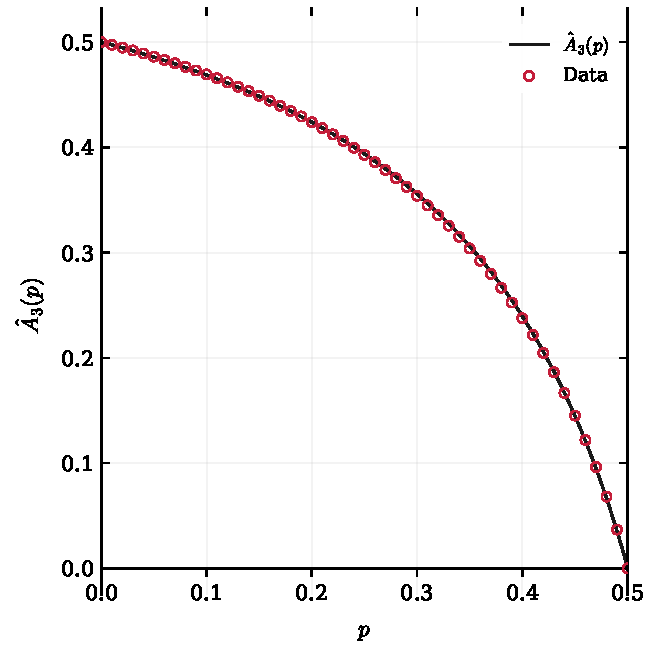
\includegraphics[width=0.6\textwidth]{figures/A3_hat_plot.pdf}
\caption{The fitted curve $\widehat A_3$ of \cref{a:eq:Ahat3} (solid) against
numerically computed values of $A(p)$ (red circles). The agreement is excellent
to the eye across the whole interval, which is exactly the problem: the fit is not
evidence of correctness. $\widehat A_3$ misses the critical point, returning
$\widehat A_3(\tfrac12)\approx9.1\times10^{-4}$ rather than $0$, and arrives
there with gradient approximately $-3.63$ instead of $-4$. Errors of this size are
invisible here but are fatal for $1/A$ near criticality.}
\label{a:fig:A3hat}
\end{figure}

\subsection{Splicing the critical branch}
\label{a:app:splice}

One can force the correct critical branch by splicing the asymptotic onto a fitted
curve:
\begin{equation}
\widehat A_4(p)
=
\begin{cases}
-0.04011483983619545\,\ee^{\ee^{2p}}
  +0.6079994336528085,
  &p<0.499962,\\[1mm]
2-4p,
  &p\ge0.499962.
\end{cases}
\label{a:eq:Ahat4}
\end{equation}
This is a practical surrogate, not a closed form for $A$. If a splice is needed,
the certified product of \cref{a:eq:partialproduct,a:eq:tailbound} is preferable
on the first branch and the proved asymptotic \cref{a:thm:nearcrit} on the
second; that is the construction adopted in \cref{a:sec:practical}.

% --- restore default section numbering for subsequent chapters --------------
\renewcommand{\thesection}{\thechapter.\arabic{section}}
